% Options for packages loaded elsewhere
\PassOptionsToPackage{unicode}{hyperref}
\PassOptionsToPackage{hyphens}{url}
\PassOptionsToPackage{dvipsnames,svgnames,x11names}{xcolor}
%
\documentclass[
  letterpaper,
  DIV=11,
  numbers=noendperiod]{scrartcl}

\usepackage{amsmath,amssymb}
\usepackage{iftex}
\ifPDFTeX
  \usepackage[T1]{fontenc}
  \usepackage[utf8]{inputenc}
  \usepackage{textcomp} % provide euro and other symbols
\else % if luatex or xetex
  \usepackage{unicode-math}
  \defaultfontfeatures{Scale=MatchLowercase}
  \defaultfontfeatures[\rmfamily]{Ligatures=TeX,Scale=1}
\fi
\usepackage{lmodern}
\ifPDFTeX\else  
    % xetex/luatex font selection
\fi
% Use upquote if available, for straight quotes in verbatim environments
\IfFileExists{upquote.sty}{\usepackage{upquote}}{}
\IfFileExists{microtype.sty}{% use microtype if available
  \usepackage[]{microtype}
  \UseMicrotypeSet[protrusion]{basicmath} % disable protrusion for tt fonts
}{}
\makeatletter
\@ifundefined{KOMAClassName}{% if non-KOMA class
  \IfFileExists{parskip.sty}{%
    \usepackage{parskip}
  }{% else
    \setlength{\parindent}{0pt}
    \setlength{\parskip}{6pt plus 2pt minus 1pt}}
}{% if KOMA class
  \KOMAoptions{parskip=half}}
\makeatother
\usepackage{xcolor}
\usepackage[top=20mm,bottom=20mm,left=20mm,right=20mm]{geometry}
\setlength{\emergencystretch}{3em} % prevent overfull lines
\setcounter{secnumdepth}{-\maxdimen} % remove section numbering
% Make \paragraph and \subparagraph free-standing
\makeatletter
\ifx\paragraph\undefined\else
  \let\oldparagraph\paragraph
  \renewcommand{\paragraph}{
    \@ifstar
      \xxxParagraphStar
      \xxxParagraphNoStar
  }
  \newcommand{\xxxParagraphStar}[1]{\oldparagraph*{#1}\mbox{}}
  \newcommand{\xxxParagraphNoStar}[1]{\oldparagraph{#1}\mbox{}}
\fi
\ifx\subparagraph\undefined\else
  \let\oldsubparagraph\subparagraph
  \renewcommand{\subparagraph}{
    \@ifstar
      \xxxSubParagraphStar
      \xxxSubParagraphNoStar
  }
  \newcommand{\xxxSubParagraphStar}[1]{\oldsubparagraph*{#1}\mbox{}}
  \newcommand{\xxxSubParagraphNoStar}[1]{\oldsubparagraph{#1}\mbox{}}
\fi
\makeatother


\providecommand{\tightlist}{%
  \setlength{\itemsep}{0pt}\setlength{\parskip}{0pt}}\usepackage{longtable,booktabs,array}
\usepackage{calc} % for calculating minipage widths
% Correct order of tables after \paragraph or \subparagraph
\usepackage{etoolbox}
\makeatletter
\patchcmd\longtable{\par}{\if@noskipsec\mbox{}\fi\par}{}{}
\makeatother
% Allow footnotes in longtable head/foot
\IfFileExists{footnotehyper.sty}{\usepackage{footnotehyper}}{\usepackage{footnote}}
\makesavenoteenv{longtable}
\usepackage{graphicx}
\makeatletter
\def\maxwidth{\ifdim\Gin@nat@width>\linewidth\linewidth\else\Gin@nat@width\fi}
\def\maxheight{\ifdim\Gin@nat@height>\textheight\textheight\else\Gin@nat@height\fi}
\makeatother
% Scale images if necessary, so that they will not overflow the page
% margins by default, and it is still possible to overwrite the defaults
% using explicit options in \includegraphics[width, height, ...]{}
\setkeys{Gin}{width=\maxwidth,height=\maxheight,keepaspectratio}
% Set default figure placement to htbp
\makeatletter
\def\fps@figure{htbp}
\makeatother
% definitions for citeproc citations
\NewDocumentCommand\citeproctext{}{}
\NewDocumentCommand\citeproc{mm}{%
  \begingroup\def\citeproctext{#2}\cite{#1}\endgroup}
\makeatletter
 % allow citations to break across lines
 \let\@cite@ofmt\@firstofone
 % avoid brackets around text for \cite:
 \def\@biblabel#1{}
 \def\@cite#1#2{{#1\if@tempswa , #2\fi}}
\makeatother
\newlength{\cslhangindent}
\setlength{\cslhangindent}{1.5em}
\newlength{\csllabelwidth}
\setlength{\csllabelwidth}{3em}
\newenvironment{CSLReferences}[2] % #1 hanging-indent, #2 entry-spacing
 {\begin{list}{}{%
  \setlength{\itemindent}{0pt}
  \setlength{\leftmargin}{0pt}
  \setlength{\parsep}{0pt}
  % turn on hanging indent if param 1 is 1
  \ifodd #1
   \setlength{\leftmargin}{\cslhangindent}
   \setlength{\itemindent}{-1\cslhangindent}
  \fi
  % set entry spacing
  \setlength{\itemsep}{#2\baselineskip}}}
 {\end{list}}
\usepackage{calc}
\newcommand{\CSLBlock}[1]{\hfill\break\parbox[t]{\linewidth}{\strut\ignorespaces#1\strut}}
\newcommand{\CSLLeftMargin}[1]{\parbox[t]{\csllabelwidth}{\strut#1\strut}}
\newcommand{\CSLRightInline}[1]{\parbox[t]{\linewidth - \csllabelwidth}{\strut#1\strut}}
\newcommand{\CSLIndent}[1]{\hspace{\cslhangindent}#1}

\usepackage{fvextra}
\usepackage{float}
\DefineVerbatimEnvironment{Highlighting}{Verbatim}{breaklines,commandchars=\\\{\}}
\pagenumbering{gobble}
\KOMAoption{captions}{tableheading}
\makeatletter
\@ifpackageloaded{caption}{}{\usepackage{caption}}
\AtBeginDocument{%
\ifdefined\contentsname
  \renewcommand*\contentsname{Table of contents}
\else
  \newcommand\contentsname{Table of contents}
\fi
\ifdefined\listfigurename
  \renewcommand*\listfigurename{List of Figures}
\else
  \newcommand\listfigurename{List of Figures}
\fi
\ifdefined\listtablename
  \renewcommand*\listtablename{List of Tables}
\else
  \newcommand\listtablename{List of Tables}
\fi
\ifdefined\figurename
  \renewcommand*\figurename{Figure}
\else
  \newcommand\figurename{Figure}
\fi
\ifdefined\tablename
  \renewcommand*\tablename{Table}
\else
  \newcommand\tablename{Table}
\fi
}
\@ifpackageloaded{float}{}{\usepackage{float}}
\floatstyle{ruled}
\@ifundefined{c@chapter}{\newfloat{codelisting}{h}{lop}}{\newfloat{codelisting}{h}{lop}[chapter]}
\floatname{codelisting}{Listing}
\newcommand*\listoflistings{\listof{codelisting}{List of Listings}}
\makeatother
\makeatletter
\makeatother
\makeatletter
\@ifpackageloaded{caption}{}{\usepackage{caption}}
\@ifpackageloaded{subcaption}{}{\usepackage{subcaption}}
\makeatother

\ifLuaTeX
  \usepackage{selnolig}  % disable illegal ligatures
\fi
\usepackage{bookmark}

\IfFileExists{xurl.sty}{\usepackage{xurl}}{} % add URL line breaks if available
\urlstyle{same} % disable monospaced font for URLs
\hypersetup{
  colorlinks=true,
  linkcolor={blue},
  filecolor={Maroon},
  citecolor={Blue},
  urlcolor={Blue},
  pdfcreator={LaTeX via pandoc}}


\author{}
\date{}

\begin{document}


\section{\texorpdfstring{American Lobster
(\emph{\texttt{Homarus\ americanus}})}{American Lobster (Homarus americanus)}}\label{american-lobster-homarus-americanus}

\subsection{Summary Scores}\label{summary-scores}

\begin{itemize}
\tightlist
\item
  \textbf{Sensitivity:} High - Very High
\item
  \textbf{Exposure:} Moderate
\item
  \textbf{Vulnerability:} Moderate
\end{itemize}

\begin{figure}[H]

\centering{

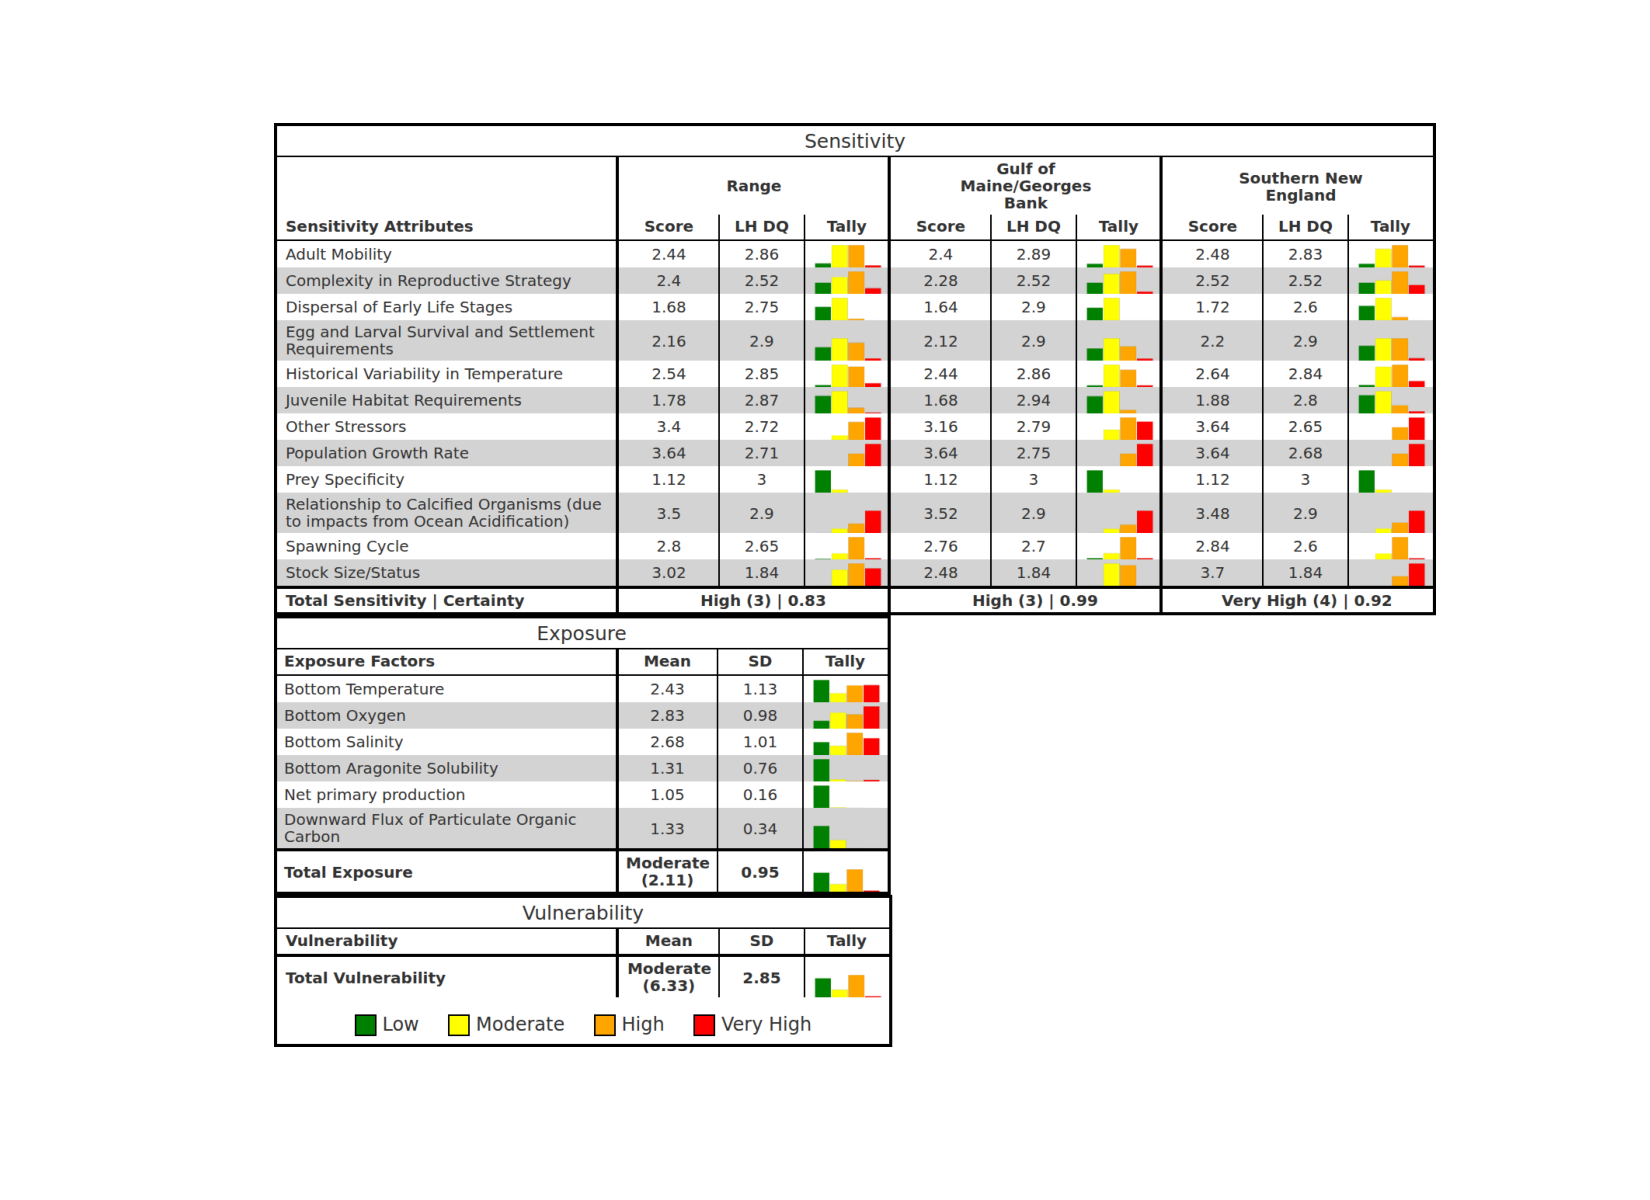
\includegraphics[width=1\textwidth,height=\textheight]{../figures/American Lobster/combined_table_allvars_r20250715_20142023_r20250925_i202501.pdf}

}

\caption{\label{fig-sum-tab-lobster}Summary Sensitivity, Exposure, and
Vulnerability Scores and Score Distributions for American Lobster.
Exposure and Vulnerability scores are averaged spatially across the
species distribution and within stocks if applicable (see
Figure~\ref{fig-vuln-lobster} and Figure~\ref{fig-exp-lobster}). Life
History Data Quality (LH DQ) and Standard Deviations (SD) are reported
for senstivity and exposure/vulnerability scores, respectively.}

\end{figure}%

\newpage{}

\subsection{Changes from Previous
Assessment(s)}\label{changes-from-previous-assessments}

\begin{longtable}[]{@{}
  >{\raggedright\arraybackslash}p{(\columnwidth - 6\tabcolsep) * \real{0.2603}}
  >{\raggedright\arraybackslash}p{(\columnwidth - 6\tabcolsep) * \real{0.2329}}
  >{\raggedright\arraybackslash}p{(\columnwidth - 6\tabcolsep) * \real{0.2740}}
  >{\raggedright\arraybackslash}p{(\columnwidth - 6\tabcolsep) * \real{0.2329}}@{}}
\caption{Changes to Vulnerability, Exposure, and Sensitivity scores
relative to Previous Assessments. If a citation for the previous
assessment is not provided, it comes from Hare et al.
(2016).}\tabularnewline
\toprule\noalign{}
\begin{minipage}[b]{\linewidth}\raggedright
Metric
\end{minipage} & \begin{minipage}[b]{\linewidth}\raggedright
Previous Assessment(s)
\end{minipage} & \begin{minipage}[b]{\linewidth}\raggedright
Current Assessment
\end{minipage} & \begin{minipage}[b]{\linewidth}\raggedright
Change
\end{minipage} \\
\midrule\noalign{}
\endfirsthead
\toprule\noalign{}
\begin{minipage}[b]{\linewidth}\raggedright
Metric
\end{minipage} & \begin{minipage}[b]{\linewidth}\raggedright
Previous Assessment(s)
\end{minipage} & \begin{minipage}[b]{\linewidth}\raggedright
Current Assessment
\end{minipage} & \begin{minipage}[b]{\linewidth}\raggedright
Change
\end{minipage} \\
\midrule\noalign{}
\endhead
\bottomrule\noalign{}
\endlastfoot
\emph{Sensitivity} & Moderate & High - Very High & Increase \\
\emph{Exposure} & High & Moderate & Decrease \\
\emph{Vulnerability} & Moderate & Moderate & None \\
\emph{Directional Effect} & Neutral & Negative & Decrease \\
\end{longtable}

\newpage{}

\subsection{Stocks}\label{stocks}

American Lobster is managed as a single stock or stock information was
not considered for this iteration of the CVA.

\subsection{Score Descriptions:}\label{score-descriptions}

\subsubsection{Sensitivity:}\label{sensitivity}

\begin{figure}[H]

\centering{

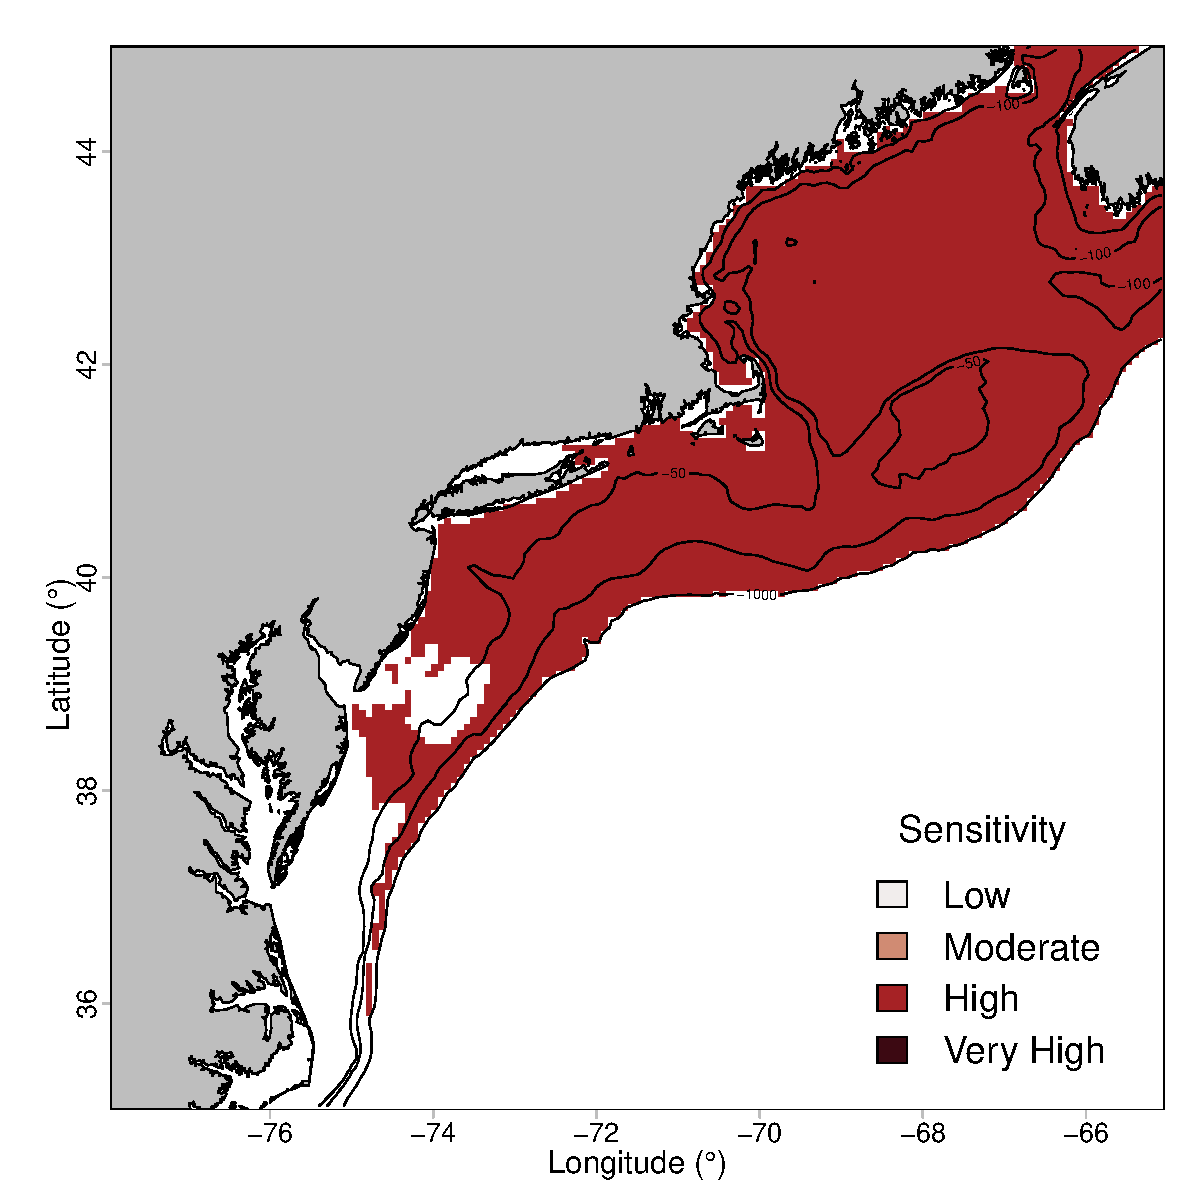
\includegraphics[width=0.85\textwidth,height=\textheight]{../figures/American Lobster/AmericanLobster_sensitivity_2.0.pdf}

}

\caption{\label{fig-sens-lobster}American Lobster Sensitivity on the
Northeast Shelf}

\end{figure}%

The \textbf{Gulf of Maine/Georges Bank} stock of American lobster
received a \textbf{High} sensitivity score and the \textbf{Southern New
England} stock scored \textbf{Very High.} Certainty was high for both
stocks, with 99\% certainty for the Gulf of Maine/Georges Bank stock and
92\% certainty for the Southern New England stock
(Figure~\ref{fig-sum-tab-lobster}).

Population growth rate and other stressors drove the scores for both
stocks. Relationships to calcified organisms contributed to the High
score for the Gulf of Maine/Georges Bank stock, and received a score of
3.5 for the Southern New England stock. Stock size had the highest score
for the Southern New England Stock (Figure~\ref{fig-sum-tab-lobster}).

Lobsters are long-lived, slow growing species that can reach ages of 50+
years. Disease and the introduction of new predators such as black sea
bass and spiny dogfish impact lobsters across their range (Atlantic
States Marine Fisheries Commission (ASMFC) 2025; Goldstein et al. 2025).
American lobsters are omnivores but diets are dominated by mollusks
(Elner and Campbell 1987), which are likely to be impacted by ocean
acidification.

Sensitivity has increased since the last assessment, where lobsters
received a Moderate score. Population growth rate and other stressors
drove scores in both assessments (Hare et al. 2016).

\subsubsection{Exposure:}\label{exposure}

\begin{figure}[H]

\centering{

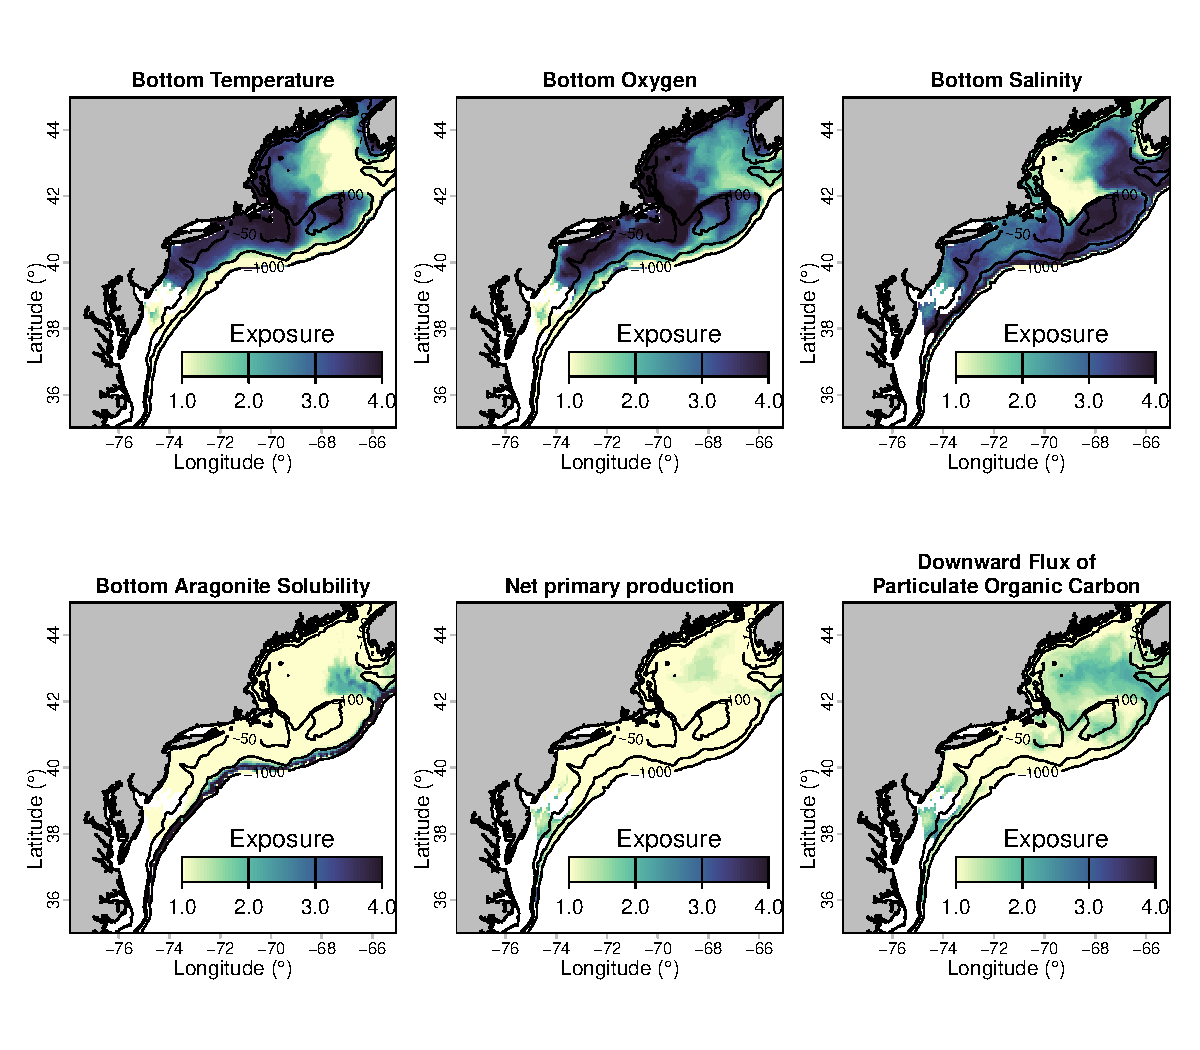
\includegraphics[width=0.85\textwidth,height=\textheight]{../figures/American Lobster/variable_exposure_maps_r20250925_i202501_r20250715_20142023.pdf}

}

\caption{\label{fig-fact-exp-lobster}Maps of each Exposure Factor for
American Lobster. Exposure was calculated between 2014-2023 and
2025-2035}

\end{figure}%

Mean exposure for American lobster across its range was
\textbf{Moderate} (2.11 +/- 0.95) (Figure~\ref{fig-sum-tab-lobster}).
Exposure was Very High over Georges Bank and High in Southern New
England and along the coast of the Gulf of Maine. Exposure was also High
along the continental shelf break (Figure~\ref{fig-exp-lobster}). These
patterns were driven by bottom temperature, oxygen, salinity, and
aragonite saturation exposure (Figure~\ref{fig-fact-exp-lobster}).

In the previous Assessment, American lobster received a High exposure
score driven by sea surface temperature and ocean acidification (Hare et
al. 2016).

\begin{figure}[H]

\centering{

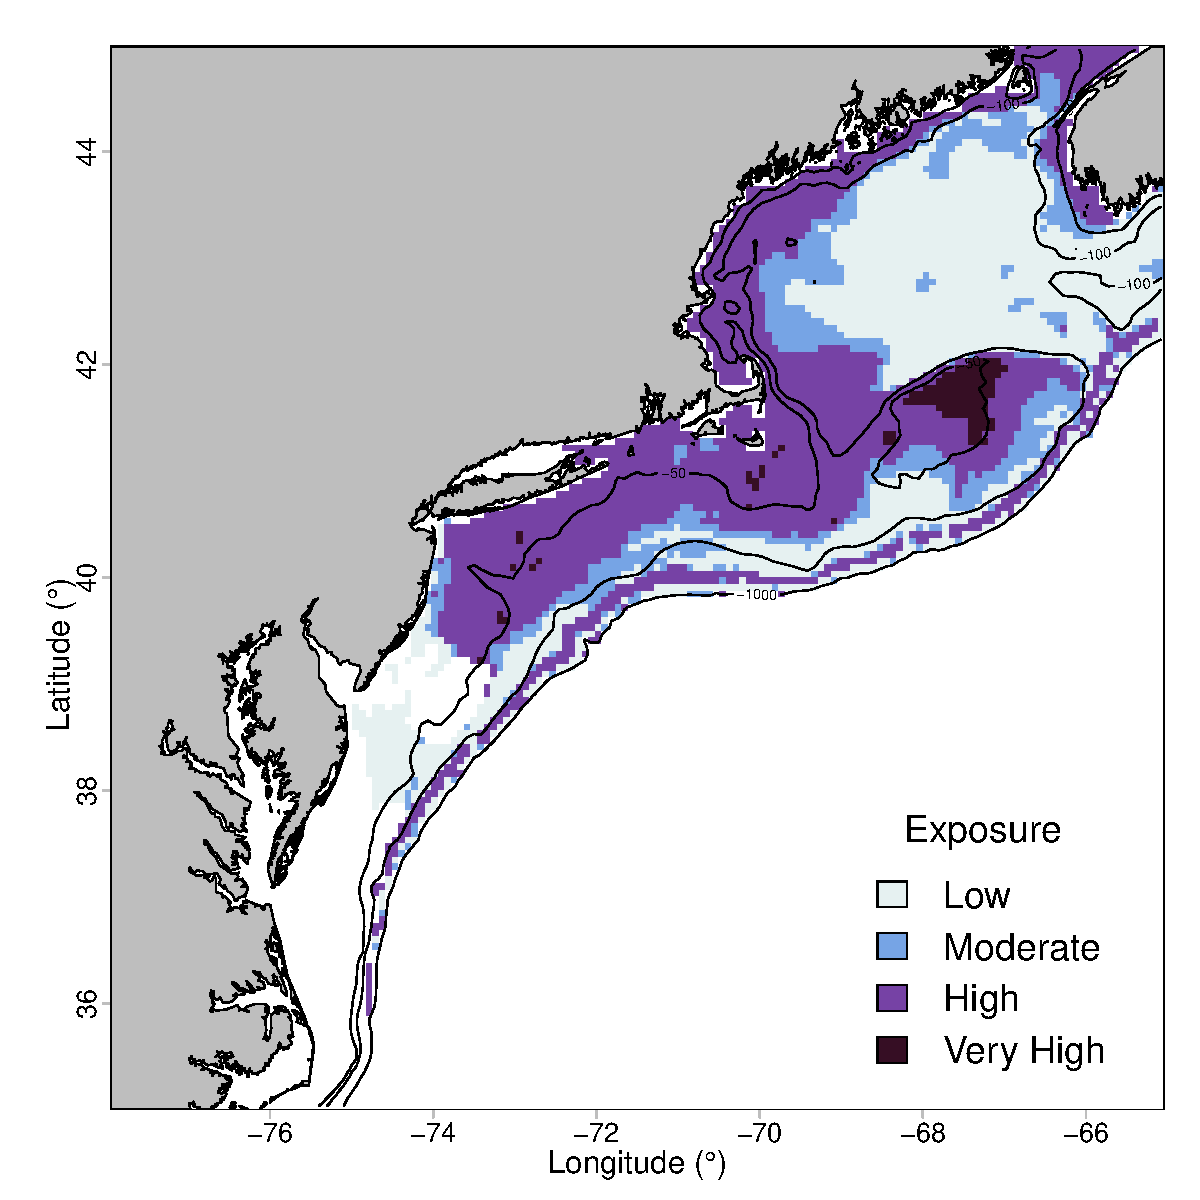
\includegraphics[width=0.85\textwidth,height=\textheight]{../figures/American Lobster/total_exposure_map_only_all_var_r20250925_i202501_r20250715_20142023.pdf}

}

\caption{\label{fig-exp-lobster}Total Exposure on the Northeast Shelf
for American Lobster. Total Exposure is calculated by applying the logic
rule from Hare et al. (2016) within grid cells across exposure factors
(see Figure~\ref{fig-fact-exp-lobster})}

\end{figure}%

\subsubsection{Vulnerability:}\label{vulnerability}

\begin{figure}[H]

\centering{

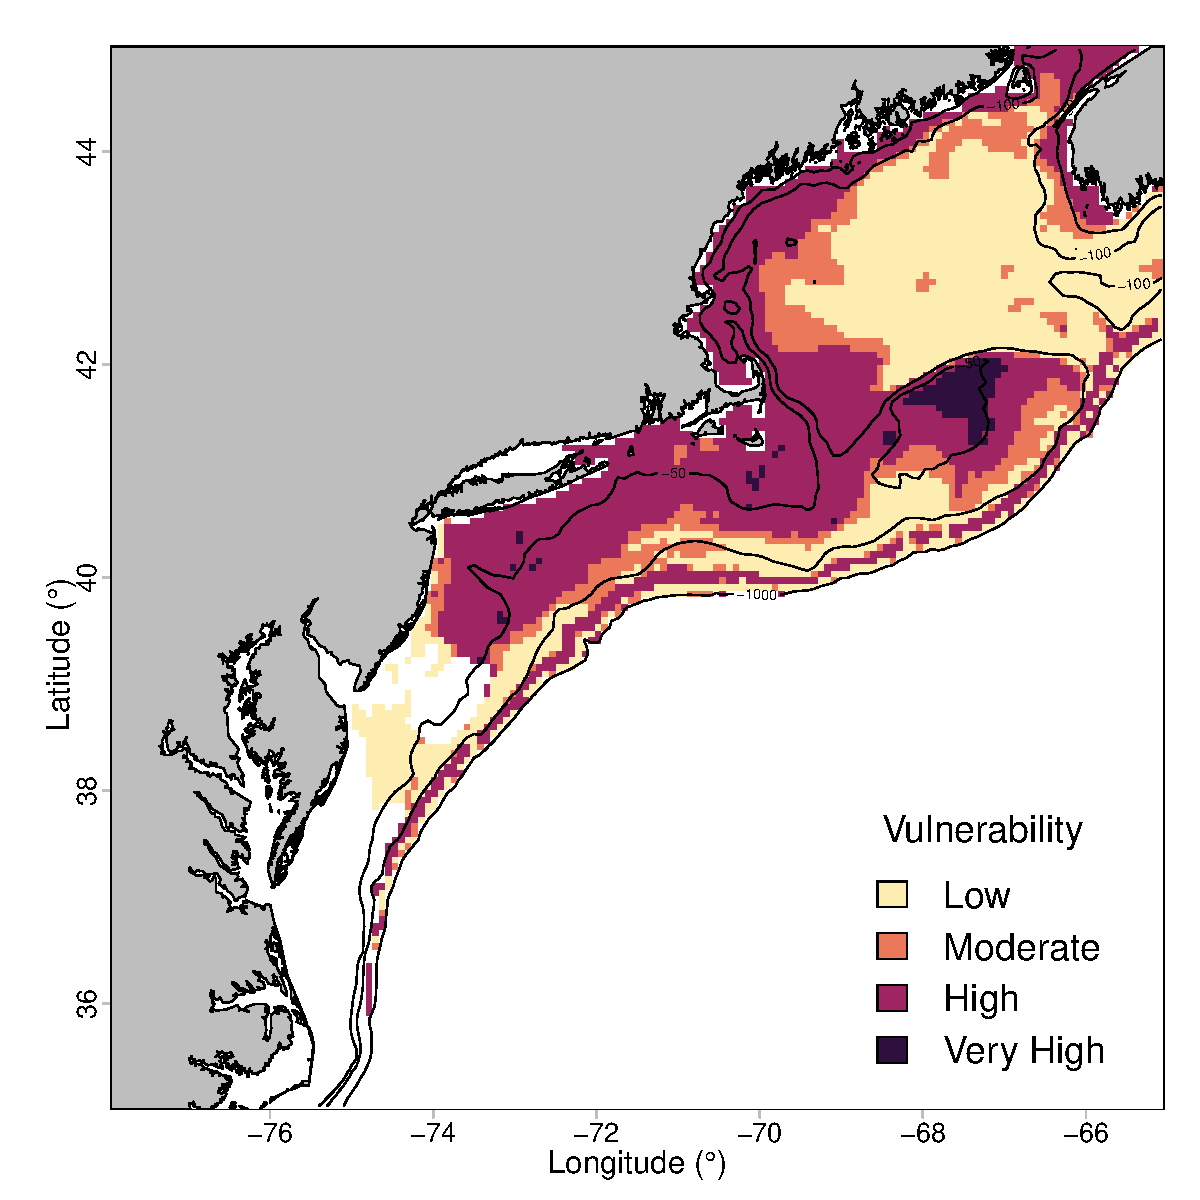
\includegraphics[width=0.85\textwidth,height=\textheight]{../figures/American Lobster/total_vulnerability_map_only_all_var_r20250925_i202501_r20250715_20142023.pdf}

}

\caption{\label{fig-vuln-lobster}Vulnerability on the Northeast Shelf
for American Lobster. Vulnerability is the product of sensitivity and
exposure (see Figure~\ref{fig-exp-lobster} and
Figure~\ref{fig-sens-lobster})}

\end{figure}%

Mean vulnerability for the American lobster was \textbf{Moderate} (6.33
+/- 2.85) across its range (Figure~\ref{fig-sum-tab-lobster}).
Vulnerability was Very High over Georges Bank and High along the coast
of the Gulf of Maine, in Southern New England, and along the continental
shelf break (Figure~\ref{fig-vuln-lobster}).

In the previous Assessment, American lobster also received a Moderate
Vulnerability score (Hare et al. 2016).

\subsection{Data Quality Metrics}\label{data-quality-metrics}

\subsubsection{Life History Data
Quality:}\label{life-history-data-quality}

The percent of data quality scores greater than 2 was 97\% for the Gulf
of Maine/Georges Bank stock and 95\% for the Southern New England stock,
indicating excellent data quality. For both stocks, Stock Size/Status
was the only data gap (mean attribute data quality score \textless{} 2)
(Figure~\ref{fig-sum-tab-lobster}).

\subsubsection{Model Confidence Score:}\label{model-confidence-score}

The mean model confidence score for American Lobster was 1.45 (+/-
0.45), indicating that experts had low confidence in the model. Experts
stated that the model missed seasonal inshore and offshore migrations.
The ensemble model's AUC was 0.86, indicating good predictive
performance.

\subsection{Additional Metrics}\label{additional-metrics}

\subsubsection{Distribution Shifts:}\label{distribution-shifts}

\begin{figure}[H]

\centering{

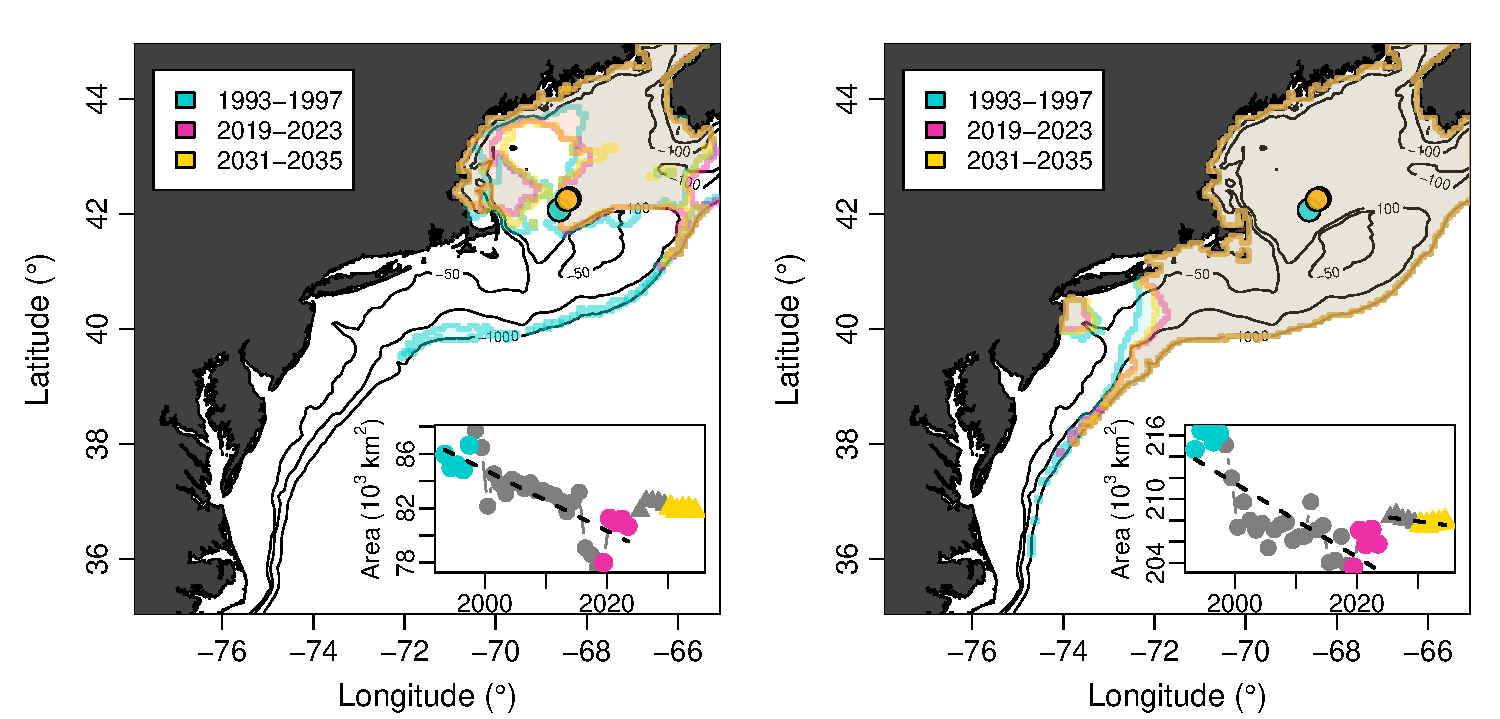
\includegraphics[width=0.85\textwidth,height=\textheight]{../figures/American Lobster/distribution_shifts_static_r20250715_r20250925_i202501.pdf}

}

\caption{\label{fig-shifts-lobster}Distribution shifts on the Northeast
Shelf for American Lobster. Polygons illustrate core habitat (left) and
species range (right) for five-year average periods. Points illustrate
weighted centroid, calculated as the average position with species
distribution models as weights. Inset timeseries illustrate the shift in
core and habitat range area over time. Circles represent points from the
MOM6 hindcast; triangles represent points from the MOM6 forecast. Dashed
lines represent significant linear regressions}

\end{figure}%

\emph{Note: For an animated version of this plot, please see the online
version of this document.}

Between 1993 and 2023, the weighted centroid shifted nearly 29 km
northeast. There were significant declines in lobster habitat along the
southern and western edges of their distribution
(Figure~\ref{fig-shifts-lobster}).

The American lobster weighted centroid is predicted to shift 4.5 km
west-southwest under near future ocean conditions. Distributions are
expected to expand westward and south (Figure~\ref{fig-shifts-lobster}).

\begin{longtable}[]{@{}
  >{\raggedright\arraybackslash}p{(\columnwidth - 10\tabcolsep) * \real{0.1667}}
  >{\raggedright\arraybackslash}p{(\columnwidth - 10\tabcolsep) * \real{0.1667}}
  >{\raggedright\arraybackslash}p{(\columnwidth - 10\tabcolsep) * \real{0.1667}}
  >{\raggedright\arraybackslash}p{(\columnwidth - 10\tabcolsep) * \real{0.1667}}
  >{\raggedright\arraybackslash}p{(\columnwidth - 10\tabcolsep) * \real{0.1667}}
  >{\raggedright\arraybackslash}p{(\columnwidth - 10\tabcolsep) * \real{0.1667}}@{}}
\caption{Distribution shifts based on five-year average distributions.
Changes are calculated relative to the previous time
period.}\tabularnewline
\toprule\noalign{}
\begin{minipage}[b]{\linewidth}\raggedright
Time Period
\end{minipage} & \begin{minipage}[b]{\linewidth}\raggedright
Weighted Centroid Shift (km \& bearing)
\end{minipage} & \begin{minipage}[b]{\linewidth}\raggedright
Core Habitat Area (change) (km\textsuperscript{2})
\end{minipage} & \begin{minipage}[b]{\linewidth}\raggedright
Habitat Total Area (change) (km\textsuperscript{2})
\end{minipage} & \begin{minipage}[b]{\linewidth}\raggedright
Latitude Range (change) (deg)
\end{minipage} & \begin{minipage}[b]{\linewidth}\raggedright
Change in Longitude Range (deg)
\end{minipage} \\
\midrule\noalign{}
\endfirsthead
\toprule\noalign{}
\begin{minipage}[b]{\linewidth}\raggedright
Time Period
\end{minipage} & \begin{minipage}[b]{\linewidth}\raggedright
Weighted Centroid Shift (km \& bearing)
\end{minipage} & \begin{minipage}[b]{\linewidth}\raggedright
Core Habitat Area (change) (km\textsuperscript{2})
\end{minipage} & \begin{minipage}[b]{\linewidth}\raggedright
Habitat Total Area (change) (km\textsuperscript{2})
\end{minipage} & \begin{minipage}[b]{\linewidth}\raggedright
Latitude Range (change) (deg)
\end{minipage} & \begin{minipage}[b]{\linewidth}\raggedright
Change in Longitude Range (deg)
\end{minipage} \\
\midrule\noalign{}
\endhead
\bottomrule\noalign{}
\endlastfoot
1993-1997 & NA & 85,851 & 215,882 & 4.74 & 7.30 \\
2019-2023 & 28.6 km NE & 80,403 (-5,447) & 205,927 (-9,955) & 4.36
(-0.37) & 6.73 (-0.56) \\
2031-2035 & 4.5 km WSW & 81,912 (+1,509) & 207,712 (+1,784) & 4.36 (0) &
6.81 (+0.08) \\
\end{longtable}

\subsubsection{Directional Effect:}\label{directional-effect}

Both stocks are likely to be \textbf{negatively} impacted by climate
change (certainties range from 81 -- 100\% based on bootstrap analysis
of expert scores). Increased thermal stress and disease will continue to
decrease the productivity of the stocks. In addition, new demersal
predators such as black sea bass and spiny dogfish will increase
predation pressures of juvenile and adult lobster. The directional
effect was estimated to be neutral in the previous Assessment (Hare et
al. 2016).

\subsection{Climate Effects on Abundance and
Distribution}\label{climate-effects-on-abundance-and-distribution}

The Northwest Atlantic has been warming at an exceptionally fast rate
(Saba et al. 2016), which has contributed to declines in fecundity and
population size in Southern New England (Goldstein, Zarrella-Smith, and
Pugh 2022) while the fishery in the central Gulf of Maine has increased
dramatically (Le Bris et al. 2018). Temperatures have increased in the
lobster's inshore range, and evidence suggests that the productivity of
the stock is severely compromised with increased thermal stress and
disease (Atlantic States Marine Fisheries Commission (ASMFC) 2025). The
assemblage of predators of American lobster has shifted with warming
conditions in the Gulf of Maine, with benthic and demersal predators,
such as black sea bass (\emph{Centropristis striata}) and spiny dogfish
(\emph{Squalus acanthias}) becoming increasingly present throughout the
lobster's range, taking the place of traditional predators, such as
Atlantic cod (\emph{Gadus morhua}). The effects of invasive and
range-expanding species may also lead to greater predation risk for
juvenile lobsters (Goldstein et al. 2025).

\subsection{Life History Synopsis}\label{life-history-synopsis}

American lobsters inhabit the coastal and oceanic waters of the Atlantic
Ocean from Labrador to North Carolina. They are widely distributed
within most of the coastal waters in the Northeast U.S. with some major
offshore concentrations along the outer edge of the Continental Shelf
and upper slope between Georges Bank and Delaware Bay (Mackenzie and
Moring 1985). Spawning takes place during a 4 month period from late May
through much of September, when females leave their solitary shelters
about 7 days before molting to share the shelter of a dominant male
(Factor 1995) (Mackenzie and Moring 1985). Lobster larvae are planktonic
for 6-8 weeks (Factor 1995) and travel from surface waters offshore to
inshore areas of Southern New England and the Gulf of Maine. Larval
distribution is affected by the distribution of spawning females and by
surface current velocity and direction, temperature, salinity, light
intensity, and hydrostatic pressure (Katz, Cobb, and Spaulding 1994)
(Harding and Trites 1988) (Hudson and Fradette 1993; Mackenzie and
Moring 1985). Larval survival is likely affected by pollution of the
marine environment by human activity, especially coastal waters (Connor
1972). There is an inverse relationship between temperature and the time
from hatching to the postlarval stage (when they settle). Larvae take as
few as 11 days at 22°C and as many as 54 days at 10°C to reach the
postlarval stage. It is speculated that thermoclines are a negative cue
for larvae/post larvae settlement (Factor 1995; Templeman 1936).
Juvenile lobsters utilize shelters (rocks and vegetation) in the benthic
habitat, and may also burrow in mud (Wahle and Steneck 1991). Juveniles
are omnivorous but also scavenge for food. Much of their diet consists
of bottom invertebrates, crabs, urchins, mussels, polychaetes,
periwinkles, and sea stars, but they may also consume fish and plants
(Lawton 1987). Adult lobsters are also considered omnivores and
scavengers . However, their diet is dominated by mollusks (especially
mussels), echinoderms, and polychaetes (Elner and Campbell 1987).
Juveniles and adults prefer bottom water temperatures of 8-14°C
(Mackenzie and Moring 1985). Inshore, adult lobsters appear to have a
limited home range of about 2.2 km, however offshore lobsters tend to
migrate greater distances (up to 345 km in 71 days) (Mackenzie and
Moring 1985). American lobster are managed by the Atlantic States Marine
Fisheries Commission as three stock units based on life history
differences: Gulf of Maine, Georges Bank, and southern New England
(Atlantic States Marine Fisheries Commission (ASMFC) 2025).

\subsection{Supplemental Scores}\label{supplemental-scores}

\subsubsection{Exposure Timeseries}\label{exposure-timeseries}

\begin{figure}[H]

\centering{

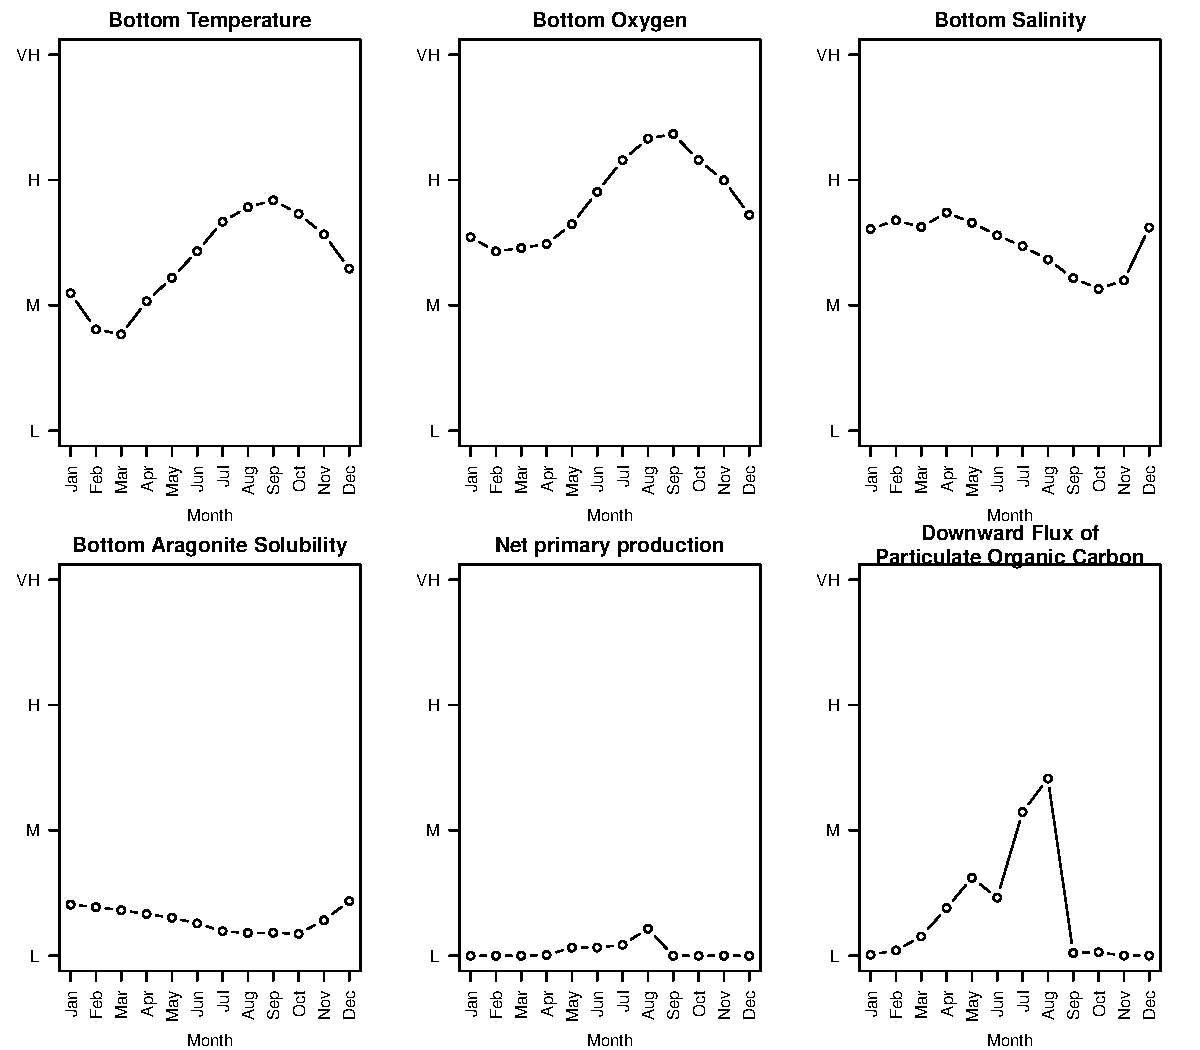
\includegraphics[width=0.85\textwidth,height=\textheight]{../figures/American Lobster/variable_exposure_timeseries_r20250925_i202501_r20250715_20142023.pdf}

}

\caption{\label{fig-exp-month-tm-lobster}Monthly Timeseries of each
Exposure Factor for American Lobster. Exposure was calculated between
2014-2023 and 2025-2035}

\end{figure}%

Monthly exposure scores ranged from Moderate to Low
(Figure~\ref{fig-exp-month-lobster}). Scores were Low from February to
April, corresponding to a decline in bottom temperature and oxygen
exposure (Figure~\ref{fig-exp-month-lobster},
Figure~\ref{fig-exp-month-tm-lobster}). Scores were Moderate for the
remainder of the year (Figure~\ref{fig-exp-month-lobster}).

\begin{figure}[H]

\centering{

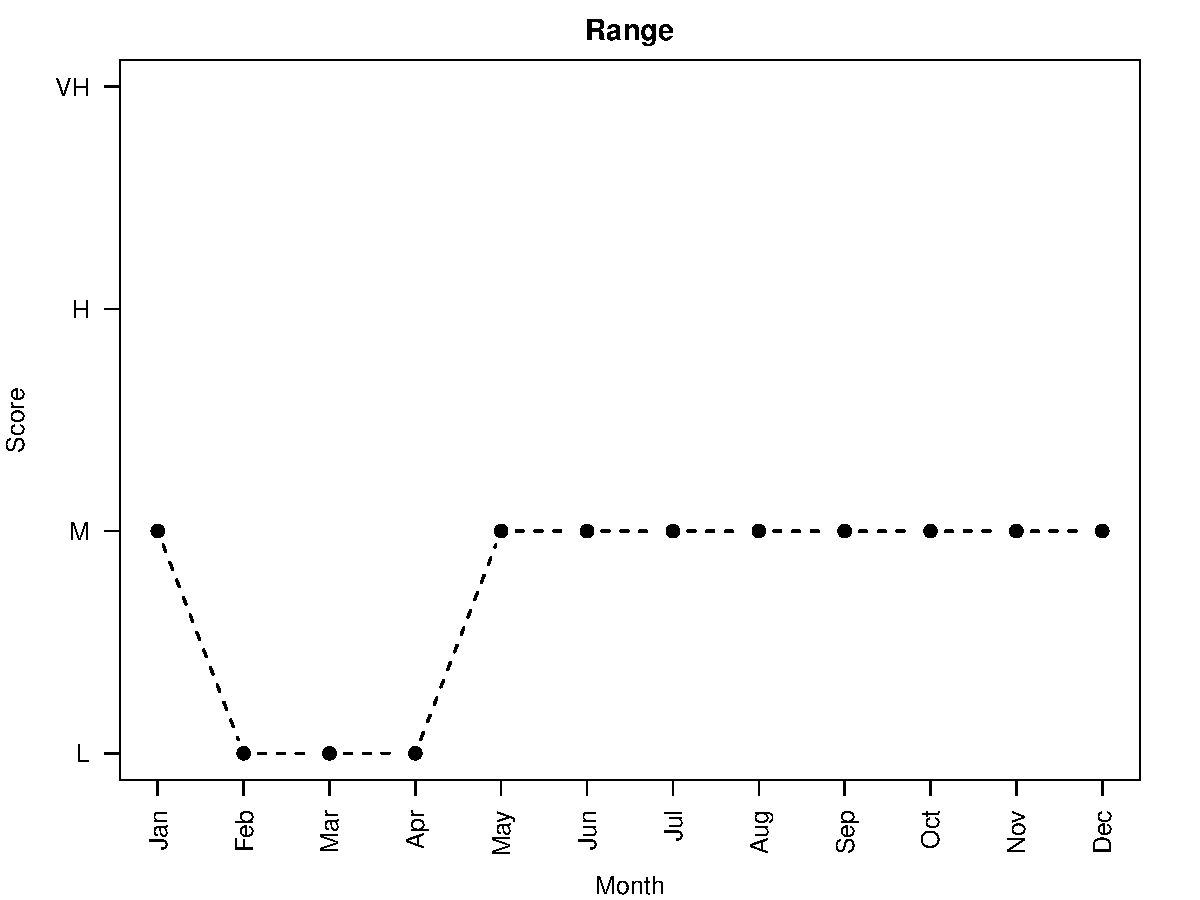
\includegraphics[width=0.85\textwidth,height=\textheight]{../figures/American Lobster/total_exposure_timeseries_only_all_var_r20250925_i202501_r20250715_20142023.pdf}

}

\caption{\label{fig-exp-month-lobster}Timeseries of Total Exposure for
American Lobster}

\end{figure}%

\subsubsection{Exposure due to Significant
Factors}\label{exposure-due-to-significant-factors}

\begin{figure}[H]

\centering{

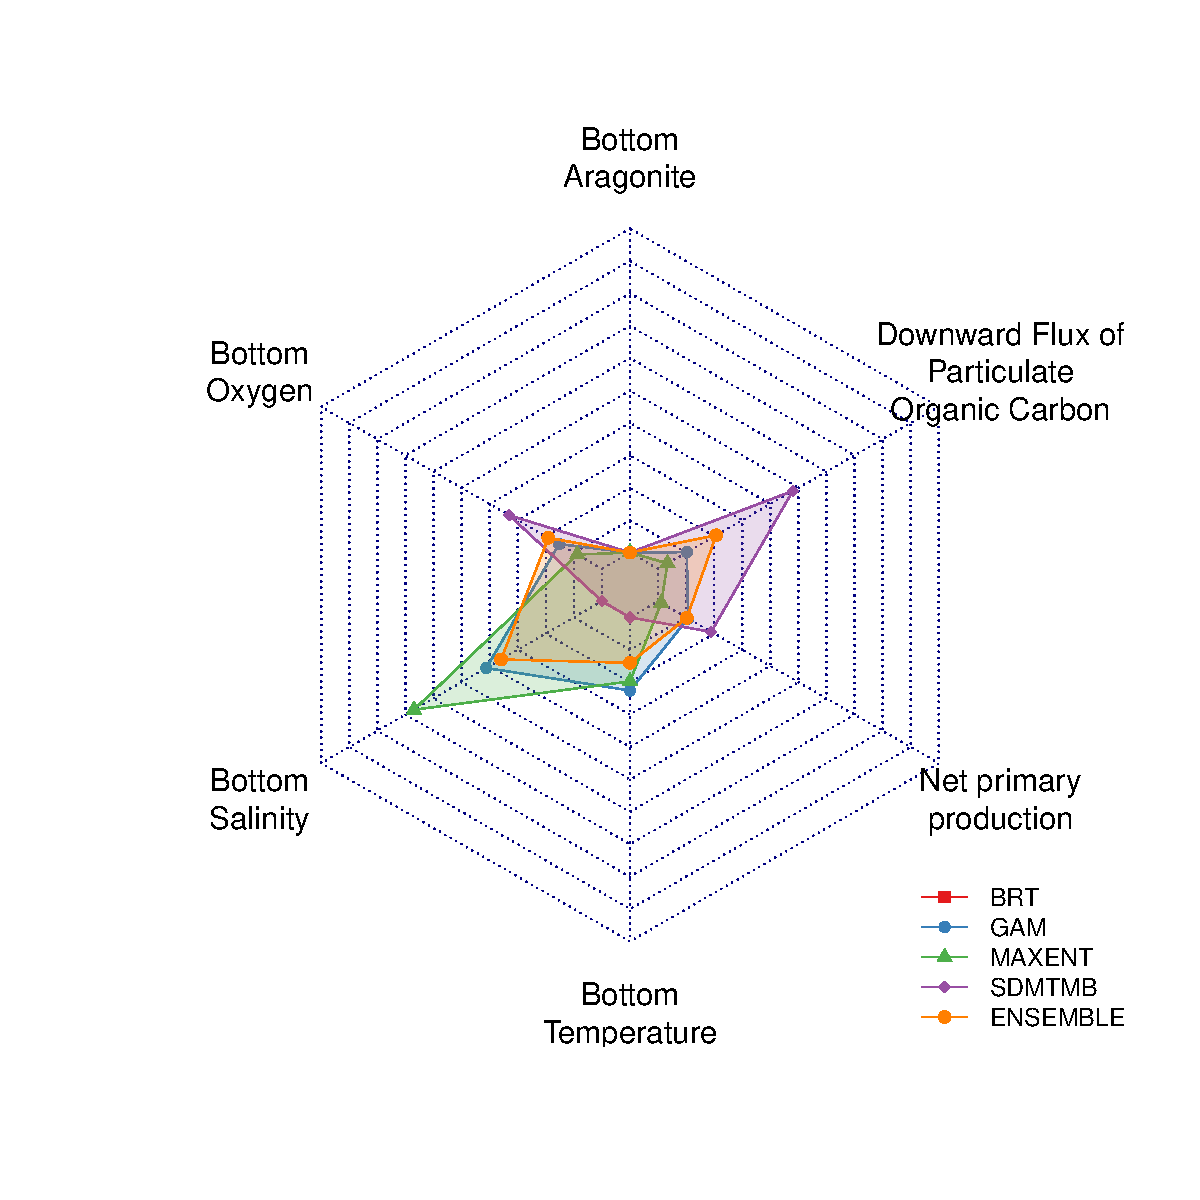
\includegraphics[width=0.85\textwidth,height=\textheight]{../figures/American Lobster/dynamic_variable_importance_r20250715.pdf}

}

\caption{\label{fig-radar-lobster}Dynamic Factors driving American
Lobster distributions. The closer the polygon is to the edge of the
figure, the more important the variable is. Each ring represents 10\%
variance explained. Factors must explain at least 10\% of variance in
the ensemble model to be used to calculate total exposure.}

\end{figure}%

Bottom temperature, oxygen, and salinity, in addition to net primary
production and downward carbon flux were all important dynamic drivers
of lobster distributions (Figure~\ref{fig-radar-lobster}). Lobsters are
omnivorous scavengers (Elner and Campbell 1987). They prefer colder
waters and utilize rocky and vegetative habitats for cover (Wahle and
Steneck 1991). When only these factors were used to calculate exposure,
scores remained Moderate (1.99 +/- 0.96)
(Figure~\ref{fig-sum-imp-lobster}, Figure~\ref{fig-exp-imp-lobster}).

\begin{figure}[H]

\centering{

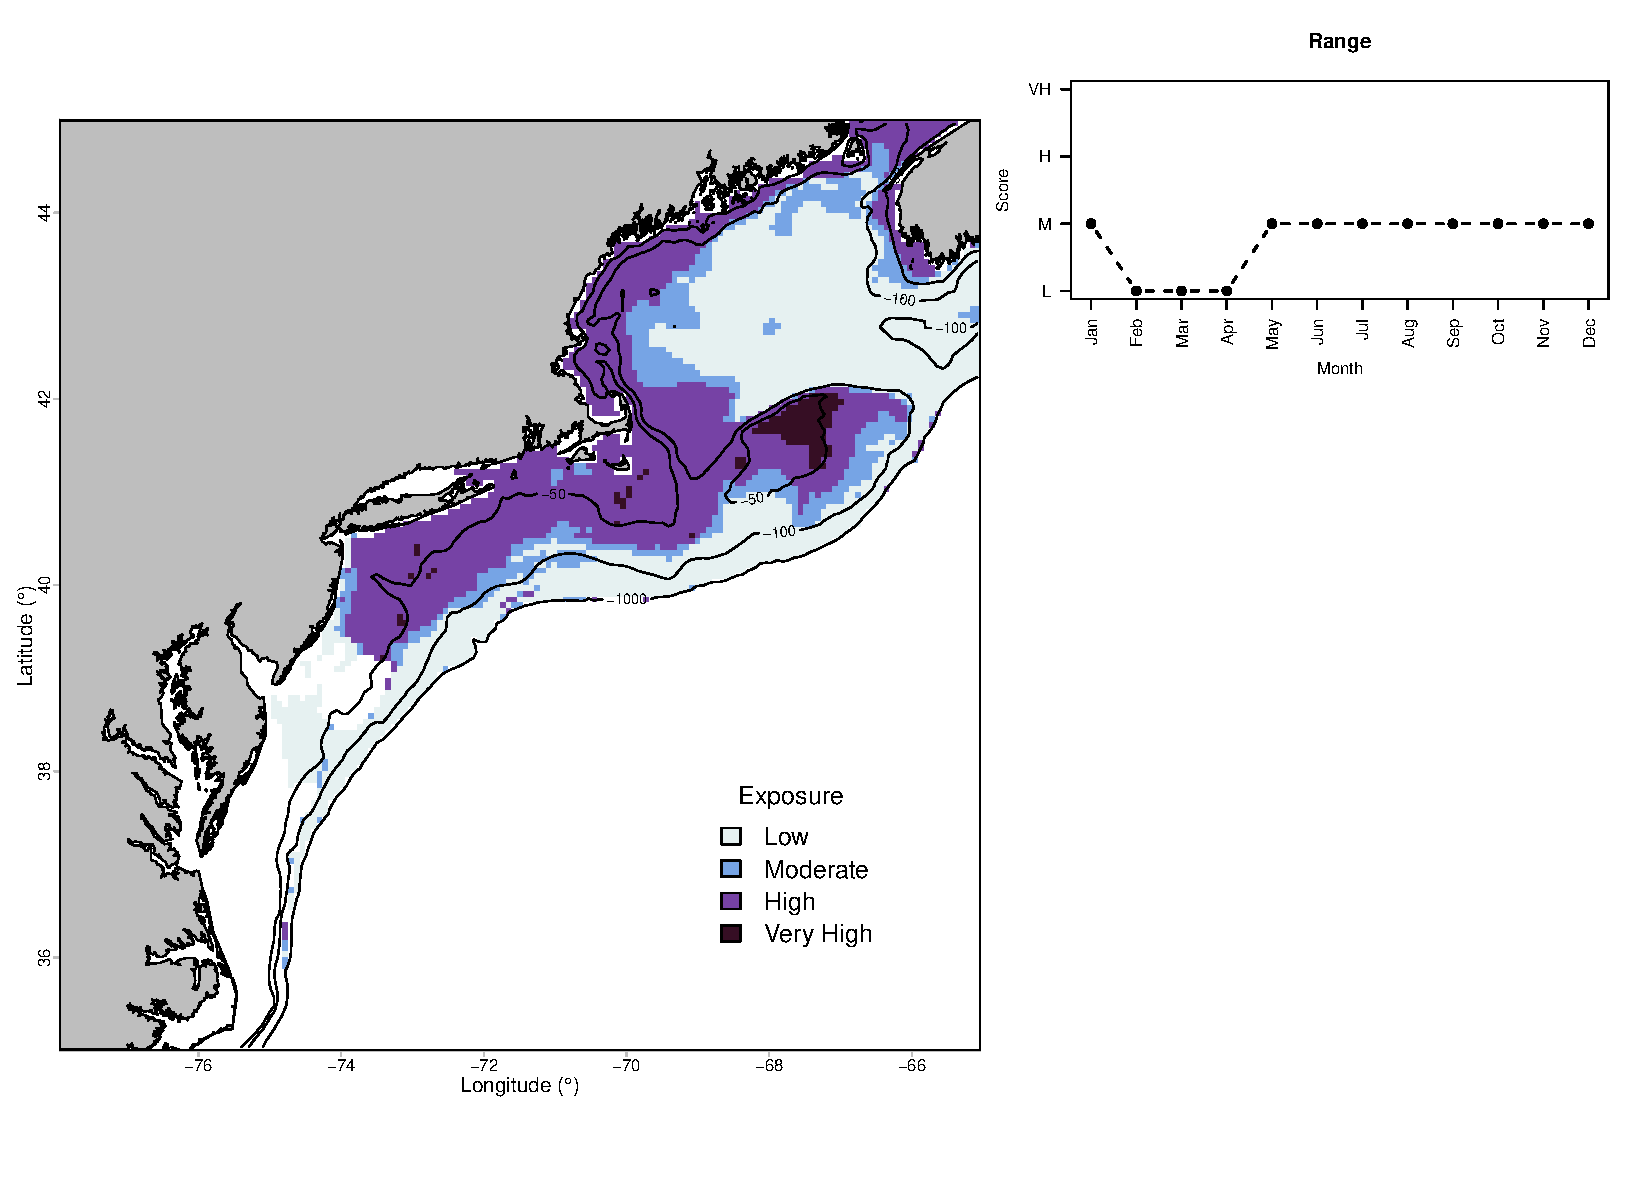
\includegraphics[width=0.85\textwidth,height=\textheight]{../figures/American Lobster/total_exposure_map_timeseries_imp_var_r20250925_i202501_r20250715_20142023.pdf}

}

\caption{\label{fig-exp-imp-lobster}Total Exposure Map and Timeseries
when Exposure was calculated with only Exposure Factors critical to
American Lobster distributions}

\end{figure}%

\begin{figure}[H]

\centering{

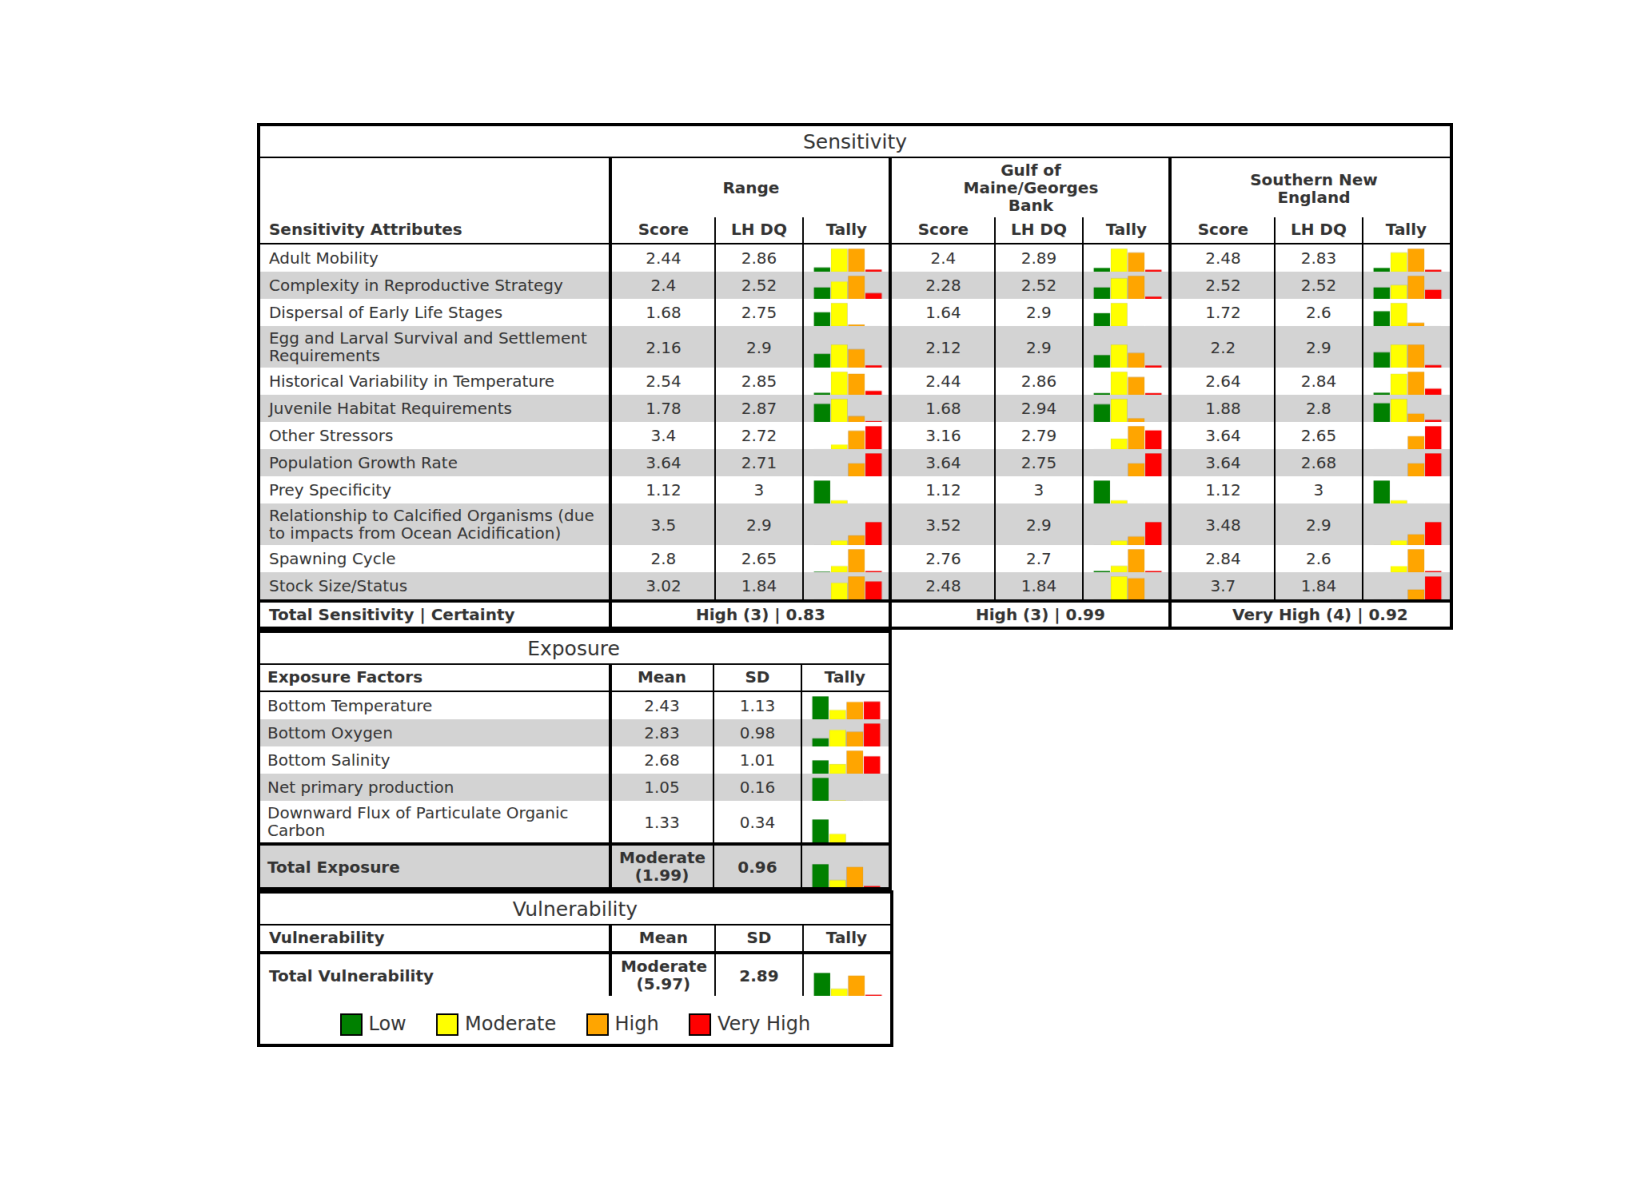
\includegraphics[width=1\textwidth,height=\textheight]{../figures/American Lobster/combined_table_impvars_r20250715_20142023_r20250925_i2025012.pdf}

}

\caption{\label{fig-sum-imp-lobster}As in
Figure~\ref{fig-sum-tab-lobster} for American Lobster, but with only
significant Exposure factors and the resulting Vulnerability Scores.}

\end{figure}%

\subsection*{References}\label{references}
\addcontentsline{toc}{subsection}{References}

\phantomsection\label{refs}
\begin{CSLReferences}{1}{0}
\bibitem[\citeproctext]{ref-asmfc2025}
Atlantic States Marine Fisheries Commission (ASMFC). 2025. {``ASMFC
Stock Assessment Overview: American Lobster.''} Atlantic States Marine
Fisheries Commission.
\url{https://asmfc.org/wp-content/uploads/2025/11/AmericanLobsterStockAssmtOverview_Oct2025.pdf}.

\bibitem[\citeproctext]{ref-connor1972}
Connor, P. M. 1972. {``Acute Toxicity of Heavy Metals to Some Marine
Larvae.''} \emph{Marine Pollution Bulletin} 3: 190--92.
\url{https://doi.org/10.1016/0025-326X(72)90234-8}.

\bibitem[\citeproctext]{ref-elner1987}
Elner, R. W., and A. Campbell. 1987. {``Natural Diets of Lobster
{Homarus} Americanus from Barren Ground and Macroalgal Habitats Off
Southwestern {Nova Scotia}, {Canada}.''} \emph{Marine Ecology Progress
Series} 37: 131--40.

\bibitem[\citeproctext]{ref-factor1995}
Factor, J. R. 1995. \emph{Biology of Lobster: {Homarus} Americanus}.
Academic Press, Inc.

\bibitem[\citeproctext]{ref-goldstein2025}
Goldstein, J. S., B. C. Gutzler, A. S. Kough, J. T. Carloni, A. M.
Dayton, C. M. Guenther, S. H. Jury, and W. H. Watson III. 2025. {``A
Review of {American} Lobster ({Homarus} Americanus) Research Since
2000.''} \emph{Reviews in Fisheries Science \& Aquaculture} 34 (1).
\url{https://doi.org/10.1080/23308249.2025.2514440}.

\bibitem[\citeproctext]{ref-goldstein2022}
Goldstein, J. S., K. A. Zarrella-Smith, and T. L. Pugh. 2022. {``Recent
Declines in {American} Lobster Fecundity in Southern {New England}:
Drivers and Implications.''} \emph{ICES Journal of Marine Science} 79
(5): 1662--74. \url{https://doi.org/10.1093/icesjms/fsac083}.

\bibitem[\citeproctext]{ref-harding1988}
Harding, G. C., and K. W. Trites. 1988. {``Dispersal of {Homarus}
Americanus Larvae in the {Gulf of Maine} from {Browns Bank}.''}
\emph{Canadian Journal of Fisheries and Aquatic Sciences} 21: 180--99.

\bibitem[\citeproctext]{ref-hare2016vulnerability}
Hare, Jonathan A, Wendy E Morrison, Mark W Nelson, Megan M Stachura,
Eric J Teeters, Roger B Griffis, Michael A Alexander, et al. 2016. {``A
Vulnerability Assessment of Fish and Invertebrates to Climate Change on
the Northeast US Continental Shelf.''} \emph{PloS One} 11 (2): e0146756.

\bibitem[\citeproctext]{ref-hudson1993}
Hudson, C., and P. Fradette. 1993. {``Wind-Induced Advection of Larval
Decapods into {Baie de Plaisance} ({Iles de la Madeleine, Quebec}).''}
\emph{Canadian Journal of Fisheries and Aquatic Sciences} 40: 1422--32.

\bibitem[\citeproctext]{ref-katz1994}
Katz, C. H., J. S. Cobb, and M. Spaulding. 1994. {``Larval Behavior,
Hydrodynamic Transport and Potential Offshore-to-Inshore Recruitment in
the {American} Lobster {Homarus} Americanus.''} \emph{Marine Ecology
Progress Series} 103: 265--73.

\bibitem[\citeproctext]{ref-lawton1987}
Lawton, P. 1987. {``Diel Activity and Foraging Behavior of Juvenile
{American} Lobsters, {Homarus} Americanus.''} \emph{Canadian Journal of
Fisheries and Aquatic Sciences} 44 (6): 1195--205.

\bibitem[\citeproctext]{ref-lebris2018}
Le Bris, A., K. E. Mills, R. A. Wahle, Y. Chen, M. A. Alexander, A. J.
Allyn, J. G. Schuetz, J. D. Scott, and A. J. Pershing. 2018. {``Climate
Vulnerability and Resilience in the Most Valuable {North American}
Fishery.''} \emph{Proceedings of the National Academy of Sciences} 115
(8): 1831--36. \url{https://doi.org/10.1073/pnas.1711122115}.

\bibitem[\citeproctext]{ref-mackenzie1985}
Mackenzie, C., and J. R. Moring. 1985. {``Species Profiles: Life
Histories and Environmental Requirements of Coastal Fishes and
Invertebrates ({North Atlantic}) {AMERICAN LOBSTER}.''} Biological
Report 82(11.33). U.S. Fish; Wildlife Service.

\bibitem[\citeproctext]{ref-saba2016}
Saba, V. S., S. M. Griffies, W. G. Anderson, M. Winton, M. A. Alexander,
T. L. Delworth, J. A. Hare, et al. 2016. {``Enhanced Warming of the
{Northwest Atlantic Ocean} Under Climate Change.''} \emph{Journal of
Geophysical Research: Oceans} 121: 118--32.
\url{https://doi.org/10.1002/2015JC011346}.

\bibitem[\citeproctext]{ref-templeman1936}
Templeman, W. 1936. {``The Influence of Temperature, Salinity, Light and
Food Conditions on the Survival and Growth of the Larvae of the Lobster
({Homarus} Americanus).''} \emph{Journal of the Biological Board of
Canada} 2: 485--97.

\bibitem[\citeproctext]{ref-wahle1991}
Wahle, R. A., and R. S. Steneck. 1991. {``Recruitment Habitats and
Nursery Grounds of the {American} Lobster {Homarus} Americanus: A
Demographic Bottleneck?''} \emph{Marine Ecology Progress Series} 69:
231--43.

\end{CSLReferences}




\end{document}
